\section{Modeling of visco-elastic environments  \label{sec:contact_mode_compliant}}

Let us now consider a rigid body that makes a contact with a visco-elastic surface, and we assume that:
\begin{enumerate}
    \item there exists an inertial frame $\mathcal{I}$;
    \item there exist a frame $B$ rigidly attached to the body and we denote $o_B$ the origin of the frame and $[B]$ its orientation;
    \item all the point of the rigid body in contact with the environment define a set denoted with $\Omega \in \mathbb{R}^3$ and named \emph{contact domain}, we denote with ${}^B x$ a point on the contact surface expressed in the frame $B$, while with ${}^\mathcal{I} x$ the very same point expressed in the inertial frame $\mathcal{I}$;
    \item the environment characteristics are isotropic;
    \item the rigid body moves with a 6D velocity, denoted as ${}^{B[\mathcal{I}]} \mathrm{v}$ such that 
    \begin{equation}
    {}^{B[\mathcal{I}]} \mathrm{v} = 
    \begin{bmatrix}
       {}^\mathcal{I}\dot{o}_B \\
       {}^\mathcal{I}\omega_{\mathcal{I},B}
    \end{bmatrix} 
    \end{equation}
   where $B[\mathcal{I}] = \left(o_B, [\mathcal{I}]\right)$ is a frame having the origin in $o_B$ and oriented as $\mathcal{I}$.
    \item  $\forall x \in \Omega$, there exists a continuous pure force distribution that depends on the point ${}^\mathcal{I} x$ and its velocity ${}^\mathcal{I} \dot{x}$, i.e.,
    \begin{equation}
        \label{eq:compliant_model_rho_definition_subscript}
        \rho_x : \mathbb{R}^3 \times \mathbb{R}^3  \rightarrow \mathbb{R}^3.
    \end{equation}
\end{enumerate}
\begin{figure}[t]
    \centering
	\includegraphics{chapter_compliant_contact/figures/2d_contact.tikz}
	\caption[The visco-elastic model: a 2D representation.]{2D representation of the visco-elastic model. The gray rectangle represents the zero-force rigid body position. The orange rectangle is the body. $\Omega$ is the contact domain while $\bar{\mathcal{X}}$ is equal to $\Omega$ if the contact wrench is null ${}_{B[\mathcal{I}]} \mathrm{f} = 0$. The interaction between the rigid body and the environment can be approximate as a continuum of spring-damper systems. }
	\label{fig:2d_contact_model}
\end{figure}
Figure~\ref{fig:2d_contact_model} shows a rigid body in contact with a visco-elastic environment.

Each point of $\Omega$ may define a different function $\rho_x$. For the sake of simplicity, we assume that $\rho_x$ is the same for each point in contact with the environment. Consequently, we drop the subscript $x$ in Equation~\eqref{eq:compliant_model_rho_definition_subscript}. 
Given the above assumptions, the contact torque distribution about a point $o_B \in \mathbb{R}^3$, $\sigma_{o_B} : \mathbb{R}^3 \times \mathbb{R}^3  \rightarrow \mathbb{R}^3$ writes
    \begin{equation}
        \sigma_{o_B}\left({}^\mathcal{I}x, {}^\mathcal{I} \dot{x}\right) = \left({}^\mathcal{I}x - o_B\right)\times \rho\left({}^\mathcal{I}x, {}^\mathcal{I} \dot{x}\right).
    \end{equation}
Once the pure force and torque distribution are defined, then the equivalent contact 6D force expressed in mixed representation is given by \citep{Caron2015StabilityAreas} -- Section~\ref{sec:zmp}:
\begin{equation}
\label{eq:compliant-contact-contact-wrench}
    {}_{B[\mathcal{I}]} \mathrm{f} = \begin{bmatrix}
    {}_\mathcal{I} f \\
    {}_{B[\mathcal{I}]} \mu
    \end{bmatrix} = 
    \begin{bmatrix}
    \int_\Omega \rho \diff \Omega \\
    \int_\Omega \sigma_{o_B} \diff \Omega \\
    \end{bmatrix}.
\end{equation}
\par
We now propose a model that can be used to describe the contact between a body and a compliant environment.
\begin{lemma}
\label{lemma:compliant_model}
Let $\bar{\mathcal{X}}$ the set of points $\bar{x}\in\mathbb{R}^3$:
\begin{equation}
     \bar{\mathcal{X}} = \{ \bar{x}\in\mathbb{R}^3  : \rho(\bar{x}, 0) = 0  \}.
\end{equation}
Assume that: $i)$ the contact domain $\Omega$ is a rectangle of dimensions $l$ and $w$; $ii)$ the point $o_B {\in} \mathbb{R}^3$ is the center of the rectangular domain;  $iii)$ the distribution $\rho$ is given by:
\begin{equation}
\rho\left({}^\mathcal{I} x, {}^\mathcal{I} \dot{x}\right) = k \left( {}^\mathcal{I} \bar{x} - {}^\mathcal{I} x\right) - b \; {}^\mathcal{I} \dot{x},
\label{eq:contact_model_general}
\end{equation}
with $k>0$ and $b>0$.
\par
Then, the equivalent contact force and torque $ {}_{B[\mathcal{I}]} \mathrm{f}$ \eqref{eq:compliant-contact-contact-wrench} are given by
\begin{IEEEeqnarray}{rcl}
\phantomsection \label{eq:contact_wrench_integral_rectangle}
 \IEEEyesnumber  \IEEEyessubnumber*
\label{eq:contact_force_integral_rectangle}
{}_\mathcal{I} f  &\;=\;& lw |e _ 3^\top \prescript{\mathcal{I}}{}R _B e _ 3| [k (\bar{o}_B - o_B) - b \dot{o}_B] \\
\label{eq:contact_torque_integral_rectangle}
{}_{B[\mathcal{I}]} \mu &=&  \frac{l w}{12} |e _ 3^\top \prescript{\mathcal{I}}{}{R} _B e _ 3| \nonumber \\
&&\left\{l^2  (\prescript{\mathcal{I}}{}{R} _B e_1) \times [b  (\prescript{\mathcal{I}}{}{R} _B e_1) \times {}^{\mathcal{I}} \omega _ {\mathcal{I},B} + k   \prescript{\mathcal{I}}{}{\bar{R}} _B e_1]  \right .  \\
&& + \left . w^2  (\prescript{\mathcal{I}}{}{R} _B e_2) \times [b  (\prescript{\mathcal{I}}{}{R} _B e_2) \times {}^{\mathcal{I}} \omega _ {\mathcal{I},B} + k   \prescript{\mathcal{I}}{}{\bar{R}} _B e_2] \right\} \nonumber,
\end{IEEEeqnarray}
where $\prescript{\mathcal{I}}{}R _B$ is the rotation from the inertial frame $\mathcal{I}$ to a frame rigidly attached to the body $B$.
$\dot{o}_B$ and ${}^{\mathcal{I}} \omega _ {\mathcal{I}, B}$ are the linear and angular velocity of the rigid body expressed in mixed representation. $\bar{o}_B$ and  $\prescript{\mathcal{I}}{}{\bar{R}} _{B}$ are the position and the rotation of the frame $B$ such that in case of zero velocity, the 6D force is null. 
\end{lemma}
The set $\bar{\mathcal{X}}$ can also be defined by considering a point $P$ that belongs to the contact domain $\Omega$ of the rigid body $B$ in contact with the compressible environment. Then, the point $P$ can move to a point $P_0$ of the space such that the force distribution at the point $P_0$ is zero. In coordinates, let $P$ be defined by the coordinate vector $x_p \in \mathbb{R}^3$ and $P_0$ be defined by the coordinate vector $\bar{x}_p \in \mathbb{R}^3$. Then given $x_p$
\begin{equation}
    \rho(\bar{x}_p, 0) = 0.
\end{equation}
$\bar{\mathcal{X}}$ contains all the points $\bar{x}_p$ associated with each point $P$ belonging to the contact domain $\Omega$.
\begin{figure}[t]
\centering
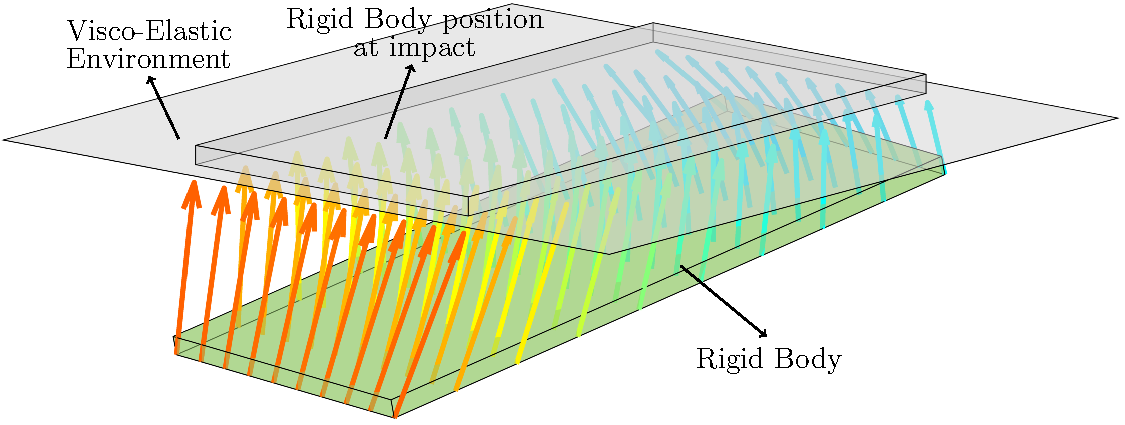
\includegraphics[width=1\columnwidth]{chapter_compliant_contact/figures/paper_fig.pdf}
\caption[Vector field generated by the visco-elastic model]{Vector field generated by the visco-elastic model -- Equation~\eqref{eq:contact_model_general}. The grey box represents the zero-force rigid-body position. The green parallelepiped is the body. The arrows represent the forces that act on the contact surface; the lighter the color, the higher the force magnitude. \label{fig:contact_model_vector_field}}
\end{figure}
The proof of Lemma~\ref{lemma:compliant_model} is in Appendix~\ref{appendix:proof_lemma_compliant}.
\par
Lemma~\ref{lemma:compliant_model} shows that the 6D contact force \eqref{eq:compliant-contact-contact-wrench} depends only on the distribution of the contact force $\rho$ on the shape of the contact domain $\Omega$ and on the rigid body state, namely \emph{position}, \emph{orientation}, \emph{linear} and \emph{angular velocity}. As a consequence, we avoid using rotational springs and dampers to describe the interaction between the robot and the environment. Furthermore, Lemma~\ref{lemma:compliant_model} also contains a close solution for the equivalent contact wrench \eqref{eq:contact_force_integral_rectangle} \eqref{eq:contact_torque_integral_rectangle} in the case of a linear contact model~\eqref{eq:contact_model_general} and a rectangular contact surface $\Omega$. As a consequence, it can be exploited in hard-real-time applications such as control architectures.
To give the reader a better understanding, we can imagine that the set $\bar{\mathcal{X}}$ contains the position of all the points on the foot sole at the touch down. Once the contact is established, the environment is deformed. The interaction between the foot and the environment is then approximated as a continuum of spring-damper systems -- Equation~\eqref{eq:contact_model_general}.
Each spring-damper system exerts a force on the associated point of the contact domain. Combining all forces, we can imagine that the rigid body is subject to the vector field represented in Figure~\ref{fig:contact_model_vector_field}. 
Finally, we want to recall that, since the contacts are unilateral, this model is valid as long as the normal forces are positive and the tangential component lies inside the friction cone.

\subsection{Linear approximation of the visco-elastic model}
It is worth noting that the model~\eqref{eq:contact_force_integral_rectangle}-\eqref{eq:contact_torque_integral_rectangle} also encompasses the classical linear modeling techniques for soft terrains. The following corollary shows, in fact, that linear approximations of~\eqref{eq:contact_force_integral_rectangle}-\eqref{eq:contact_torque_integral_rectangle} lead to linear and rotational springs and dampers that are usually used to model contact wrenches due to soft terrains~\cite[Equation~(8)]{Sygulla2020AFootholds:}.
\begin{corollary}
\label{corollary:approximation}
Let ${}_{\mathcal{I}} f$ and ${}_{B[\mathcal{I}]} \mu $ be the contact force and torque given by \eqref{eq:contact_force_integral_rectangle} and \eqref{eq:contact_torque_integral_rectangle}, respectively. Assume that $\prescript{\mathcal{I}}{}{\bar{R}} _B = I _3 $ and $\prescript{\mathcal{I}}{}{R} _B$ is approximated with its first order of the Taylor expansion, i.e., $\prescript{\mathcal{I}}{}R _B = I_3 + \Theta\times$, with $\Theta \in \mathbb{R}^3$. Assume that $\Theta$ represents the classical sequence of roll-pitch-yaw, namely $\prescript{\mathcal{I}}{}R _B(\Theta) = R_z(\Theta_3)R_y(\Theta_2)R_x(\Theta_1)$.
Then, the contact model \eqref{eq:contact_force_integral_rectangle}-\eqref{eq:contact_torque_integral_rectangle} writes 
\begin{IEEEeqnarray}{c}
\phantomsection \label{eq:linear_model}
 \IEEEyesnumber  \IEEEyessubnumber*
    {}_{\mathcal{I}} f_l = \mathcal{K}_l (\bar{o}_B - o_B) - \mathcal{B}_l \dot{o}_B, \label{eq:linear_model_force}\\ 
    {}_{B[\mathcal{I}]} \mu_l = - \mathcal{K}_a \Theta - \mathcal{B}_a \dot{\Theta} \IEEEyessubnumber* \label{eq:linear_model_torque},
\end{IEEEeqnarray}
with 
\begin{equation}
\mathcal{K}_l = l w k I_3, \quad \mathcal{K}_a =  k \frac{l w}{12} \begin{bmatrix} w ^ 2 & 0 & 0 \\ 
0 & l ^ 2 & 0 \\ 
0 & 0& l ^2 {+} w ^2 \end{bmatrix}
\end{equation}
\begin{equation}
\mathcal{B}_l = l w b I_3, \quad \mathcal{B}_a =  b \frac{l w}{12} \begin{bmatrix} w ^ 2 & 0 & 0 \\ 
0 & l ^ 2 & 0 \\ 
0 & 0& l ^2 {+} w ^2 \end{bmatrix}
\end{equation}
\end{corollary}

The proof of Corollary~\ref{corollary:approximation} is in Appendix~\ref{appendix:proof_corollary_compliant}.
Corollary~\ref{corollary:approximation} thus shows that
the model~\eqref{eq:contact_force_integral_rectangle}-\eqref{eq:contact_torque_integral_rectangle} extends the linear models~\citep{Sygulla2020AFootholds:} to the case of \emph{large} contact surface orientations. 
\par
Here, we want to underline that the classical linear approaches for modeling compliant contacts ~\eqref{eq:linear_model} -- for example, rotational springs and dampers \citep{Sygulla2020AFootholds:}~-- are often valid only for \emph{small} contact surface rotations. This is due to the minimal representation (i.e., three angles, such as \emph{roll}, \emph{pitch}, \emph{yaw}) used to represent $\SO(3)$. In addition, the equivalent \emph{rotational stiffness and dampers} values $\mathcal{K}_a$ and $\mathcal{B}_a$ are often not related to the physical parameters of the contact. On the other hand, even if the model we propose ~\eqref{eq:contact_force_integral_rectangle}-\eqref{eq:contact_torque_integral_rectangle} is indeed a 6d force, it is obtained by integrating pressure and shear stresses distributions to better catch the fundamental effects of the contact physics, without having the aforementioned issues of classical rotational spring and damper models.
\par
\begin{figure}[t]
\centering
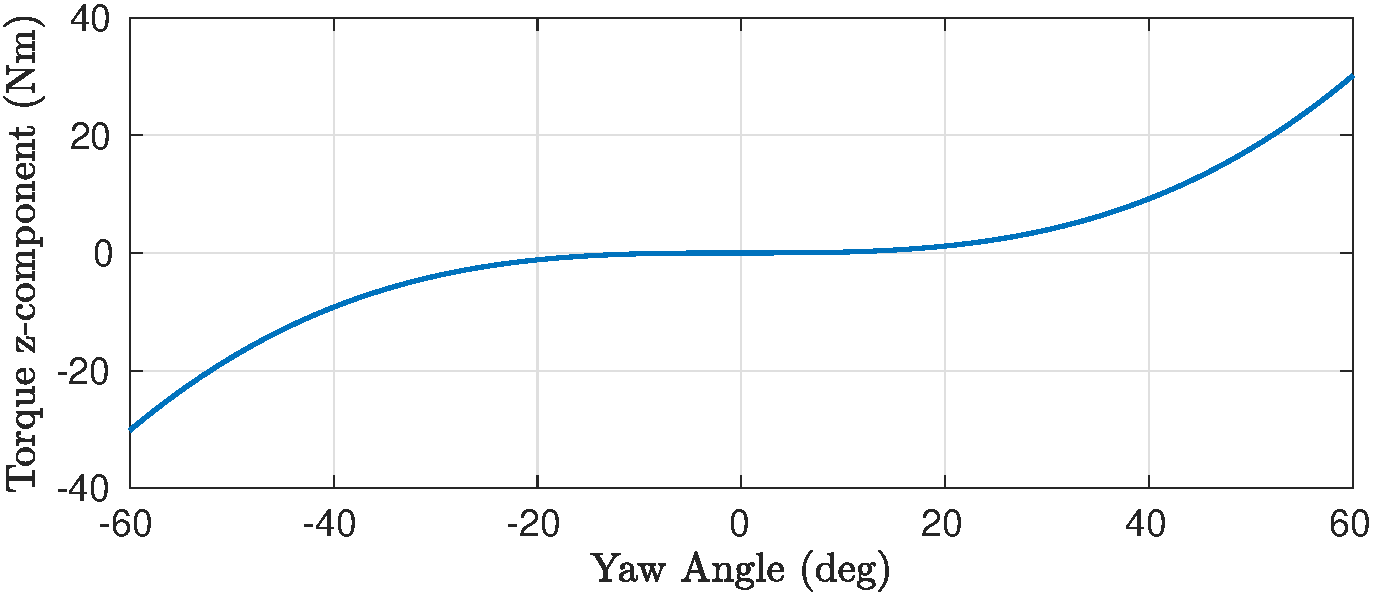
\includegraphics[width=0.9\columnwidth]{chapter_compliant_contact/figures/comparison_lumped_continuous.pdf}
\caption{Linear approximation error for different values of yaw angle.
\label{fig:approximation_error}}
\end{figure}
Let us now introduce the approximation error between the linear model~\eqref{eq:linear_model} and the model presented~\eqref{eq:contact_wrench_integral_rectangle} as $\epsilon_\mathrm{f} = {}_{B[\mathcal{I}]} \mathrm{f}  - {}_{B[\mathcal{I}]}\mathrm{f}_l$.
Figure~\ref{fig:approximation_error} shows the last component of the error $\epsilon_\mathrm{f}$, i.e., $e_6^\top \epsilon_\mathrm{f}$, in the case of zero velocity and zero pitch and roll angles. The higher the angle, the greater the difference. Thus, the higher is the angle, the less valid the linear approximation is. A similar analysis holds also for the other components of the 6D force. 
To conclude, the model presented in Lemma~\ref{lemma:compliant_model} is not equivalent to a linear lumped contact model, but it can be seen as a non-linear generalization while keeping a low mathematical complexity.



    











